\section{Die Algorithmen auf diesem Markt}
Der Vergleich der RL-Algorithmen findet auf dem in \ref{section:markov} definierten Markt statt.
Dieser Markt wird auf der Testplattform simuliert, die im Rahmen des Bachelorprojektes entwickelt wurde.
Er wird über die Gym-Schnittstelle durch die Agenten angesprochen.
Für die zu vergleichenden Algorithmen werden hauptsächlich die Implementierungen der Bibliothek \textit{Stable Baselines} verwendet. \cite{stable-baselines}
Stable Baselines ist ist eine weit verbreitete eine Open-Source RL-Bibliothek, die in Python geschrieben ist.
Sie baut auf PyTorch auf, einem der beliebtesten Deep-Learning-Frameworks, das in der Forschung weite Verbreitung findet. \cite{NEURIPS2019_9015}
Die in Stable Baselines implementierten Algorithmen entsprechen in den meisten Fällen unmittelbar den vorgeschlagenen Algorithmen der Originalpaper und zeichnen sich durch eine hohe Lesbarkeit des Codes aus.
Alle Hyperparameter sind konfigurierbar.

In dieser Untersuchung der Algorithmen wird stets von den Hyperparametern der Originalpaper ausgegangen.
Weil kaum theoretische Erkenntnisse über die Ermittlung optimaler Hyperparameter vorliegen und diese stets problemspezifisch sind, ist eine erschöpfende Optimierung der Hyperparameter nur mit erheblichem experimentellem Aufwand möglich.
Dazu müssten sehr viele Kombinationen mit jeweils mehreren Läufen durchgeführt werden, was einen nicht zu leistenden Ressourcenaufwand darstellt.
Dennoch wurden an einigen Stellen bessere Hyperparameter gefunden und Aussagen über die Algorithmen über mehrere Hyperparameterkombinationen abgesichert.

Alle Verfahren werden mit neuronalen Netzen durchgeführt, die zwei versteckte Schichten mit je 64 Neuronen haben.
Das Verhalten der Algorithmen für unterschiedliche Netzgrößen ist aber sehr ähnlich, wie die Experimente mit unterschiedlichen Netzgrößen im Bereich [noch zu erstellen] des Anhangs zeigen.
Für den Vergleich der Algorithmen werden diese zunächst innerhalb ihrer Gruppen betrachtet und auf generelle Eignung für dieses Setup geprüft.
Danach werden die Algorithmen, die sich als grundsätzlich geeignet erwiesen haben, hinsichtlich verschiedener Kriterien verglichen.

\section{DDPG und TD3}
Bei der Diskussion der Q-Learning-Verfahren beschränkt sich diese Analyse direkt auf die Verfahren, die im stetigen Raum angewendet werden.
Deep-Q-Networks mit diskreten Aktionen müssen jede einelne Aktion aus $\mathcal{A_\mathbb{N}}$ mit einem Aktionswert versehen.
Das sind bei der Konfiguration mit $p_{max}=10$ bereits 1000 Ausgabeneuronen und das Wachstumsverhalten ist kubisch in der Anzahl der Preisstufen.
Diese Eigenschaft verhindert den Einsatz für DQNs und Verfahren mit diskreten Aktionsräumen allgemein für dieses Problem.
Im Anhang zeigt Diagramm [noch zu erstellen] das Training von DQNs auf diesem Setup und bestätigt dessen Untauglichkeit.

\begin{figure}[htbp]
	\centering
	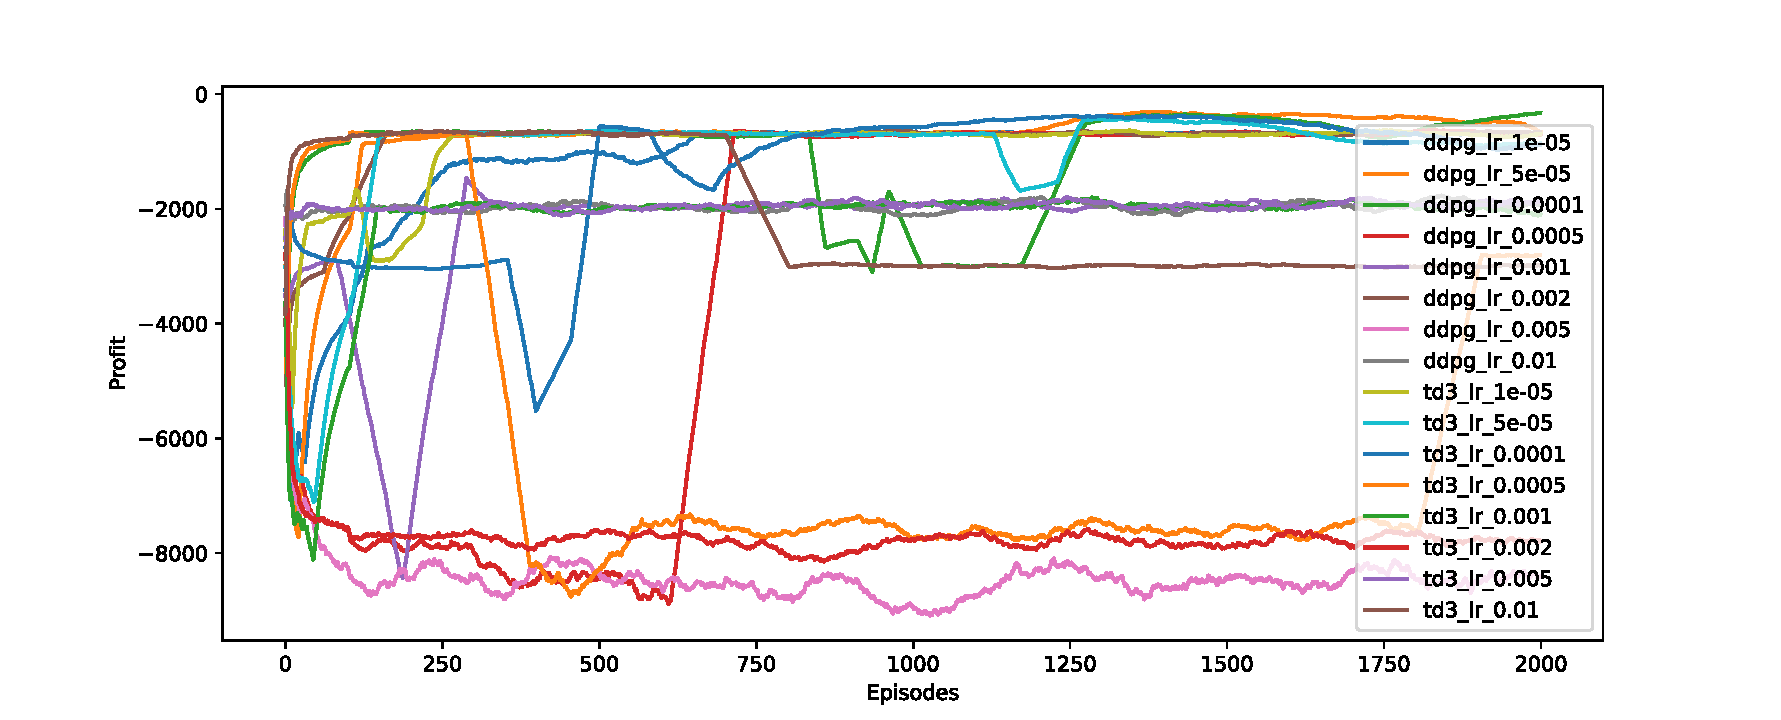
\includegraphics[width=\textwidth]{main/DDPG_learning_curve.pdf}
	\caption{Lernkurven von DDPG und TD3 mit unterschiedlichen Lernraten}
	\label{grafic:DDPGLearningCurve}
\end{figure}

Die Lernkurven der beiden sehr ähnlichen Verfahren DDPG und TD3 sind in Abbildung \ref{grafic:DDPGLearningCurve} dargestellt.
Für jeden der beiden Algorithmen wurden acht Trainingsläufe durchgeführt, die mit unterschiedlichen Lernraten parametrisiert wurden.
Der Standardwert liegt für beide Algorithmen bei $1e-3$.
Es wurden Trainingsläufe mit diesen Lernraten sowie kleineren und größeren durchgeführt.
Die beim Training beobachteten Muster gleichen sich sowohl bei den beiden Algorithmen als auch den unterschiedlichen Parametrisierungen.

Zu Beginn des Trainings ist bei einigen Läufen eine Verbesserung der gemittelten Returns, die primäre Leistungskennziffer, zu beobachten.
Allerdings kommt diese Verbesserung bei allen Algorithmen zum Erliegen und eine konstante Leistung stellt sich ein.
Dabei treten Häufungen bei der Leistung -2000 und -700 auf.
Bei einigen Trainingsdurchläufen wird ein Niveau von -300 erreicht, dieses aber nie überschritten.

Betrachtet man die Zusammensetzung der Gewinne -- die Diagramme dazu befinden sich im Anhang -- erkennt man, dass ein Teil der Agenten durch das Setzen hoher Neupreise wenige Kunden mit hoher Rendite gewinnen konnte.
Die mit dem Neuverkauf erwirtschafteten Gewinne liegen jedoch nie über 100 in der Episode und damit deutlich niedriger als bei anderen Policies.
Ein Teil der Algorithmen verharrt auf Preisen, die niedriger sind als die Einkaufspreise.
Diese ziehen besonders viele Kunden an und erhöhen dadurch noch den Verlust.
Bei der Reduktion der Rückkaufkosten konnten einige Agenten akzeptable Leistungen erreichen, aber keiner der Algorithmen konnte mit dem Verkauf gebrauchter Produkte Geld einnehmen.
Einige der Agenten mussten sogar ständig dafür Strafe zahlen, dass sie keine Gebrauchtprodukte liefern konnten.

Die Trainingsdurchläufe zeigen, dass sich die Leistung oft ruckartig verändern.
Der dabei in den Lernkurven zu erkennende lineare Auf- oder Abstieg ist der Durchschnittsbildung über die letzten hundert Episoden geschuldet.
Tatsächlich findet die Änderung sprunghaft statt, wie man es an den Scatterplots ablesen kann.
Zahlreiche der Trainingsdurchläufe sind von starken Einbrüchen der Leistung geprägt.
Diese Instabilität bei DDPG und TD3 sind als Problem bekannt.

Die Tatsache, dass die Agenten lange auf einer Stelle bleibt und auch die gleichen verbeserungswürdigen Aktionen immer wieder ausführt, kann auf unzureichende Exploration schließen lassen.
Allerdings konnten auch eine verrauschte Aktionswahl zur besseren Exploration keine Verbesserung der Leistung erreichen.

\section{On-Policy-Learning -- A2C und PPO}
Die beiden On-Policy-Verfahren A2C und PPO gibt es für diskrete wie für stetige Aktionsräume.
Wegen der großen Zahl der Aktionen wird hier jedoch nur die stetige Variante genommen.
Es wurde von den Hyperparameter ausgegangen, die in den Originalpapern vorgeschlagen wurden.
Sie finden sich auch im Anhang [genauer Abschnitt].

Grafik ? stellt die Lernkurven der Algorithmen dar.
Dabei wurde PPO mit zwei Hyperparametrisierungen verwendet, die sich im Parameter $\epsilon$ unterscheiden.
Das eine Mal wird 0,2 wie im Originalpaper verwendet, das andere Mal 0,3.
Jedes dieser Experimente wurde acht Mal unabhängig für eine Million Schritte laufen gelassen.
Die Lernkurven verwenden wieder die laufenden Durchschnitte der Episodenreturns.
Der Bereich zwischen maximalem und minimalem Episodenreturns dieser acht Agenten ist eingefärbt.
Die Linie stellt ihren Durchschnitt dar.
Obwohl die Agenten weiterhin mit starken Verlusten beginnen, stellt diese Grafik nur den Bereich zwischen 0 und 1000 dar, um durch die Skalierung einen genaueren Vergleich im oberen Leistungsbereich zu ermöglichen.

Aus den Grafiken geht unmittelbar hervor, dass alle diese Agenten die Gewinnzone erreichen.
Sie erreichen über Ergebnisse über 500, was nach den Erfahrungen mit dem regelbasierten Wettbewerber ein gutes Ergebnis darstellt.
Dabei erreichen die Advantage-Actor-Critic-Agenten das Leistungsniveau nach deutlich weniger Episoden als die PPO-Agenten.
Ihr Durchschnitt überschreitet die Schwelle zum Gewinn nach nur 110 Episoden (umgerechnet 5500 Schritte).
Dagegen ist das Training der A2C-Agenten merklich instabil.
Die Grafik ? stellt Details eines einzelnen A2C-Durchlaufes dar.
Es handelt sich dabei um einen mittleren Durchlauf, der Agent hatte sein Maximum bei 5?? und erreicht damit Platz 5 von 8.
Man sieht, dass die Aktionsauswahl permanent hin- und herschwankt.
Wie auch bei den anderen A2C-Agenten stürzt seine Leistung mitunter deutlich ab und fällt dabei weit in die Verlustzone.
Nicht immer erholen sich die Agenten davon, oft erhalten sie weiterhin schlechte Ergebnisse.
Diese heftigen Abstürze führen dazu, dass die Mittelwertlinie wieder unter 0 fällt, obwohl einige der Agenten weiterhin gute Ergebnisse liefern.

Im Gegenzug dazu ist die Trainingsstabilität bei den PPO-Varianten deutlich höher.
Zwischen den acht Trainingsdurchläufen der PPO-Agenten gibt es kaum Unterschiede in der Entwicklung.
Die Leistungsentwicklung liegt in einem schmalen Band und Abstürze finden nicht statt.
Allerdings benötigt PPO in der Standardkonfiguration etwa 5000 Episoden und in der Version mit $0,3$ als \textit{clip_range} etwa 2700 Episoden, um die Gewinnzone zu erreichen.
Auch danach ist das Training langsam.

Dieser Unterschied von PPO zu A2C überrascht nicht, er existiert \textit{by design}.
Diese Experimente zeigen, dass PPO in seiner Intention, die Trainingsstabilität zu erhöhen, erfolgreich ist.
Diese Erhöhung der Trainingsstabilität findet dadurch statt, dass die Änderung der stochastischen Policy bei den Trainingsschritten begrenzt wird.
Aus dieser Begrenzung der Policyänderung ist die geringere Lerngeschwindigkeit dann eine logische Schlussfolgerung.

So lässt sich auch erklären, warum der Durchlauf mit $\varepsilon=0,3$ schneller trainiert.
Mit größerem $\varepsilon$ wird pro Sample eine größere Policyänderung erlaubt, was zu schnellerem Training führt.
Allerdings steigt damit wieder das Risiko von Instabilität, weshalb die Parametrisierung des PPO-Algorithmus einen Trade-off zwischen Trainingsgeschwindigkeit und Stabilität eröffnet.
Die Wahl des Standardparameters $0,2$ mag in diesen Experimenten konservativ erscheinen, $0,3$ verursacht ebenfalls keine Instabilitäten.
Das Experiment ? im Anhang zeigt, wie sich PPO bei größerem $\varepsilon$ verhält.

\section{Trainingsdauer und Sample Efficiency}

\section{Stabilität}

\section{Analyse und Vergleich der ermittelten Policies}
